A neural network is a model that learns how to map fingerprints (in this case, of a molecule) to output quantities (atomization energies, spin-splitting energies).
\visible<2->{\par Nonlinear activation functions make neural networks powerful.}
\visible<3->{\par $\sigma(z)\rightarrow ReLU(z)=$\[ \begin{cases} 
z & z>0 \\
0 & otherwise
\end{cases}
\]}
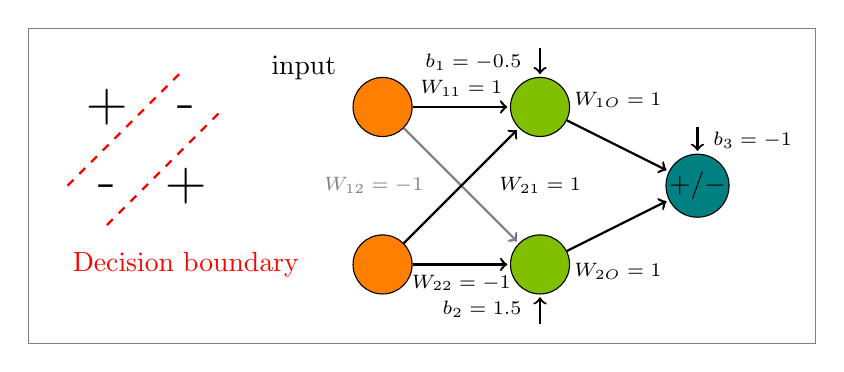
\begin{tikzpicture}[shorten >=1pt,draw=black, x=1cm, y=1 cm,  node distance=0cm]
	\draw[draw=gray, use as bounding box](-2,0) rectangle (8,4);
	\clip (-2,-0) rectangle (8,6);
	\def\layersep{2cm}
	
    \tikzstyle{every pin edge}=[<-,shorten <=1pt,thick]
    \tikzstyle{neuron}=[circle,fill=black!25,minimum size=0.75cm ,inner sep=0pt, color=black, draw]
    \tikzstyle{input neuron}=[neuron, fill=green!50!blue!50];
    \tikzstyle{output neuron}=[neuron, fill=green!50!blue];
    \tikzstyle{hidden neuron}=[neuron, fill=green!50!orange];
    \tikzstyle{annot} = [text width=2em, text centered]
    \visible<4->{\node[] (I) at (-1,2) {\huge-};}
    \visible<4->{\node[] (I) at (-1,3) {\huge+};}
    \visible<4->{\node[] (I) at (0,2) {\huge+};}
    \visible<4->{\node[] (I) at (0,3) {\huge-};}
    \visible<5->{\draw[red,thick,dashed] (-1.5,2) -- (0,3.5);}
    \visible<5->{\draw[red,thick,dashed] (-1,1.5) -- (0.5,3);}
    \visible<5->{\node[red] (I) at (0,1) {Decision boundary};}
	\visible<6->{\node[](l) at (1.5, 3.5) {input};}
	\visible<6->{\node[input neuron,fill=orange!100 ] (I-1) at (2.5,1) {$ $};}
	\visible<6->{\node[input neuron,fill=orange!100 ] (I-2) at (2.5,3) {$ $};}
	\visible<6->{\node[hidden neuron,fill=green!50!orange] (H-1) at (4.5,1) {$ $};}
	\visible<6->{\node[hidden neuron,fill=green!50!orange] (H-2) at (4.5,3) {$ $};}
	\visible<6->{\node[output neuron,fill=green!50!blue] (O) at (6.5,2) {$+/-$};}
	\foreach \dest in {1,2}{     
		\foreach \source in {1,2}{
			\visible<6->{\path[thin,->,black] (I-\source) edge node[font=\scriptsize] {} (H-\dest) ;}}
		}
	\visible<6->{\path[thin,->,black] (H-1) edge node[font=\scriptsize] {} (O);}
	\visible<6->{\path[thin,->,black] (H-2) edge node[font=\scriptsize] {} (O);}
	\visible<7->{\path[thick,->,black, midway, above,black] (I-2) edge node[font=\scriptsize] {$W_{11}=1$} (H-2) ;}
	\visible<7->{\path[thick,->,gray, midway, left,gray] (I-2) edge node[font=\scriptsize, left=10pt] {$W_{12}=-1$} (H-1) ;}
	\visible<7->{\path[thick,->,black, midway, right,black] (I-1) edge node[font=\scriptsize, right=10pt] {$W_{21}=1$} (H-2) ;}
	\visible<7->{\path[thick,->,black, midway, below,black] (I-1) edge node[font=\scriptsize] {$W_{22}=-1$} (H-1) ;}
	\visible<7->{\path[thick,->,black, midway, below,black] (H-1) edge node[font=\scriptsize, below = 10pt] {$W_{2O}=1$} (O) ;}
	\visible<7->{\path[thick,->,black, midway, below,black] (H-2) edge node[font=\scriptsize, above = 10pt] {$W_{1O}=1$} (O) ;}
	\visible<7->{\path[thick,->,black, midway, below,black] (4.5,0.25) edge node[font=\scriptsize, left = 3pt] {$b_2=1.5$} (H-1) ;}
	\visible<7->{\path[thick,->,black, midway, below,black] (4.5,3.75) edge node[font=\scriptsize, left = 3pt] {$b_1=-0.5$} (H-2) ;}
	\visible<7->{\path[thick,->,black, midway, below,black] (6.5,2.75) edge node[font=\scriptsize, right = 2pt] {$b_3=-1$} (O) ;}
\end{tikzpicture}
